\setlength{\headheight}{1.2cm}
\renewcommand{\publ}{\flushleft\footnotesize{Based on:\\[0.1cm]
		\textit{D. Sas, P. Avgeriou and F. Arcelli Fontana, "Investigating Instability Architectural Smells Evolution: An Exploratory Case Study," 2019 IEEE International Conference on Software Maintenance and Evolution (ICSME), 2019, pp. 557-567, doi: 10.1109/ICSME.2019.00090.} \\[0.1cm]
}}

\chapter{Investigating instability architectural smells evolution: an exploratory case study}\label{chap:2}
\epigraph{\emph{I've learned to always avoid saying ``always''.}}{--- Martin Fowler}


\begin{Abstract}
    Architectural smells may substantially increase maintenance effort and thus require extra attention for potential refactoring. While we currently understand this concept and have identified different types of such smells, we have not yet studied their evolution in depth. This is necessary to inform their prioritisation and refactoring.
    This study analyses the evolution of individual architectural smell \emph{instances} over time, and the \emph{characteristics} that define these instances.
    Three different types of architectural smells are taken into consideration and mined from a total of 524 versions across 14 different projects.
    The results show how different smell types differ in multiple aspects, such as their growth rate, the importance of the affected elements over time in the dependency network of the system, and the time each instance affects the system. They also cast valuable insights on what aspects are the most important to consider during prioritisation and refactoring activities.
\end{Abstract}

\section{Introduction}
In recent years, there has been increasing interest on the concept of \emph{architectural smells} (AS): issues in the architecture that often cause extra maintenance effort \cite{Lippert2006}. Several studies have explored this concept and identified different types of such smells \cite{Lippert2006,Garcia2009,Suryanarayana2014a,Mo2015}.
However, while the evolution of \emph{code} smell instances has been extensively investigated, very few studies focus on the evolution of \emph{architectural} smells and do so only at a coarse-grained level (e.g. by simply counting the number of smells in each version). There is also no work tracking the individual smell instances along system evolution.

We need to study the evolution of AS in detail because AS are a different type of ``affliction" than code smells: they usually involve more elements than code smells, they affect the system at a different scale, and they require more effort to be refactored \cite{Lippert2006}. At the same time,  the long-term advantages of this refactoring in terms of maintainability and changeability of the system are higher. Thus, the current theoretical knowledge on code smells cannot be applied to AS.

In this study, we propose an approach to study the evolution of AS detected by an open source tool named \textsc{Arcan} \cite{Arcelli2017}, by tracking individual smell instances and measuring the evolution of the properties of each detected instance. We have detected almost 150.000 unique smell instances in over 500 versions across 14 open source Java projects.
We have performed four types of analyses: a generic data mining analysis to have a better understanding of the data, a trend analysis to understand the evolution of the smells over time, a correlation analysis to identify possible correlations among the smell characteristics\footnote{See Section \ref{c2:sec:smell-characteristics} for the definition of characteristics and the full list.} considered, and a survival analysis to document their probability to persist within the system.
The focus of this study is on the architectural smells known as instability AS \cite{Arcelli2016}; these are introduced in more depth in Section \ref{c2:sec:arch-smells}.

Our findings can enable practitioners and researchers to develop strategies for optimal refactoring prioritisation of individual smell instances based on multiple factors.
For example, a Hublike dependency smell is a much better option for refactoring than a Cyclic dependency, especially in terms of complexity, and future and present maintenance effort.
Additionally, Cyclic dependencies have a much shorter lifetime on the average, making them less critical in general.

The remainder of this paper is organised as follows: Section \ref{c2:sec:related-work} discusses similar work in the literature, Section \ref{c2:sec:arch-smells} introduces the smells hereby considered, Section \ref{c2:sec:case-study} explains the methodology of this case study, Sections \ref{c2:sec:general-results}, \ref{c2:sec:rq1a-results}, \ref{c2:sec:rq1b-results}, and \ref{c2:sec:rq2-results} report and discuss the results of the different analyses, Section \ref{c2:sec:threats} lists the threats to the validity of this study and finally Section \ref{c2:sec:conclusions} concludes the paper.

\section{Related work}\label{c2:sec:related-work}
We present related work concerning both architectural smells and code smells.

In the former case, Al-Mutawa et al. \cite{AlMutawa2014} have investigated the circular (or cyclic) dependencies' shape in Java programs. 
They developed and validated a methodology to detect and classify circular dependencies starting from the bytecode of an application.
Their findings, based on a case study performed on the Qualitas Corpus \cite{QualitasCorpus2010} data set, suggest that the most common shapes (see Figure \ref{c2:fig:cycle-shapes}) are tiny and multi-hub. Moreover, they also argue that cycles among parents and children packages are less critical than cycles among non-related packages, providing empirical evidence to back up their claims.

Another study that considers the history of architectural smells was published by Roveda et al. \cite{Roveda2018}.
In their work, the authors try to estimate the architectural debt index using architectural smells and track the evolution of the index throughout a system's history.
The calculation uses partial historical information of the AS identified by the \textsc{Arcan} tool in multiple versions.
The major shortcomings of Roveda et al.'s index are:
\begin{enumerate}[label=(\roman*)]
    \item the historical information used is limited to the size of the smell and only considers the previous version,
    \item the historical information is weighted equally for every smell type, and
    \item it does not account for the \emph{magnitude} of the variation, i.e. a decrease by only one element halves the contribution of the smell to the overall index, whereas an increase by only one doubles it.
\end{enumerate}
Indeed, one of the goals of this work is also to provide theoretical background and practical tools to improve such types of calculation.

Concerning code smells, there are several works on tracking smells throughout a system's history.
In their work, Vaucher et al. \cite{Vaucher2009} have focused on the code smell God Class and its evolution in terms of the degree of \textit{``godliness"}, estimated using their previous approach based on Bayesian belief networks.
The authors analysed the trend of such a parameter for each God Class instance in the history of two systems. Their findings suggest that the godliness of God classes tends to remain constant in over 60\% of the cases.

A different perspective on code smells evolution was introduced by Chatzigeorgiou et al. \cite{Chatzigeorgiou2014}, who analysed the survival probability of four types of code smells. Their findings show that Long Methods are the most persistent code smells in the two analysed systems.

In a similar work, Peters et al. \cite{Peters2012} have also analysed the persistence of code smells in a system, though they have used a slightly less elaborate technique to do so and on a slightly different set of smells.
Their findings show that Feature Envy methods are the least persistent type of smell (similarly to the finds of Chatzigeorgiou et al.) and that Data Classes are, instead, the most persistent ones.
% Other possible RW: Tsantalis, Olbrich, Tufano

\section{Architectural smells}\label{c2:sec:arch-smells}
\subsection{Definitions and implications}
This section introduces the architectural smells (AS) considered by this dissertation. The definition of these smells is provided by Arcelli et al. \cite{Arcelli2016} and briefly reported here.

\paragraph{Unstable dependency (UD)}\label{c2:sec:arch-smells-ud}
This smell represents a component that depends upon a significant number of components that are less stable than itself.
The stability of a component is measured using Martin's instability metric \cite{Martin2018}, which measures the degree to which a component (e.g. a package) is susceptible to change based on the classes it depends upon and on the classes depending on it.
The smell thus arises when a component has a significant number of components -- the tool \textsc{Arcan} uses a 30\% threshold \cite{Arcelli2017} -- it depends upon with an instability value higher than its own.
A UD smell is detectable on Java package-like elements only (i.e. containers of classes, files, etc.). A simplified example of UD is shown in Figure \ref{c2:fig:ud}. 

The main problem caused by UD is that the probability to change the main component grows higher as the number of unstable components it depends upon grows accordingly. This increases the likelihood that the components that depend upon it (not shown in Figure \ref{c2:fig:ud} for simplicity) change as well when it is changed (ripple effect), thus inflating future maintenance efforts.

\paragraph{Hublike dependency (HL)}\label{c2:sec:arch-smells-hl}
This smell represents a component where the number of ingoing and outgoing dependencies is higher than the median in the system and the absolute difference between these ingoing and outgoing dependencies is less than a quarter of the total number of dependencies of the component \cite{Arcelli2016}. A hublike dependency can be detected both at the package and at the class level.

The implications of this smell for development activities are once again concerning the probability of change and the ease of maintenance. Consider, for example, the case represented in Figure \ref{c2:fig:hl}.
Making a change to any of the components that A depends upon may be very hard \cite{Martin2018}, even though there is only one component depending on them.
Additionally, the central component is also overloaded with responsibility and has a high coupling.
This structure is thus not desirable, as it increases the potential effort necessary to make changes to all of the elements involved in the smell.

\paragraph{Cyclic dependency (CD)}\label{c2:sec:arch-smells-cd}
This smell represents a cycle among a number of components; there are several software design principles that suggest avoiding creating such cycles \cite{Lippert2006,Parnas1979,Stevens1974,Martin2018}.
Cycles may have different topological shapes. Al-Mutawa et al. \cite{AlMutawa2014} have identified 7 of them; the ones detected by \textsc{Arcan} are shown in Figure \ref{c2:fig:cycle-shapes} \cite{Arcelli2017}.
Usually, the circle shape is intuitively perceived as the typical CD (i.e. see Figure \ref{c2:fig:cd}), but it is certainly not the only possible type of CD. In fact, there is empirical evidence \cite{AlMutawa2014} that tiny and multi-hub shapes (two stars attached together that are missing some edges) are more common than one expects.
More complex shapes mean that the cycle has lower levels of coupling and higher levels of cohesion among the elements creating the cycle.
For example, a clique-shaped cycle has the maximum amount of coupling possible with the components taking part in the cycle, drastically reducing the maintainability of the affected part of the system.

Besides affecting complexity, their presence also has an impact on compiling (causing the recompilation of big parts of the system), testing (forcing to execute unrelated parts of the system, increasing testing complexity), or deploying (forcing developers to re-deploy unchanged components) \cite{Lippert2006}.

\begin{figure}[h]
    \centering
    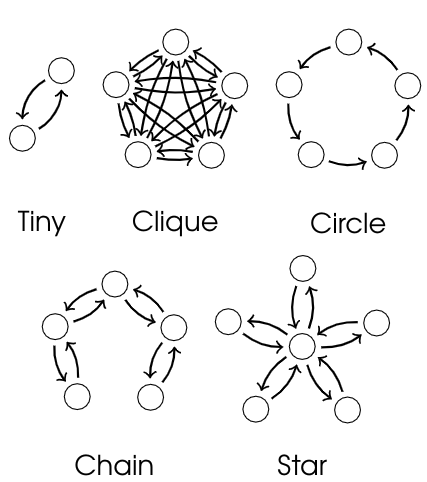
\includegraphics[width=.4\textwidth]{c4/Fig9b.png}
    \caption{Symmetric cycle shapes detected by \textsc{Arcan} and defined by Al Mutawa et al. \cite{AlMutawa2014}.}\label{c2:fig:cycle-shapes}
\end{figure}

\paragraph{God component (GC)}\label{c2:sec:arch-smells-gc}
This smell represents a component (or package, in Java) that is considerably larger in size (i.e. lines of code) than other components in the system \cite{Lippert2006} (see Figure \ref{c2:fig:gc}).
Originally, GC was defined using a fixed threshold on the lines of code, \textsc{Arcan} however uses a variable threshold-detection approach based on the frequencies of the number of lines of code of the other packages in the system \cite{Arcelli2015}.

God components aggregate too many concerns together in a single artefact and they are generally a sign that there is a missing opportunity for splitting up the component into multiple sub-components.
God components tend to become such over time, as a result of several little incremental changes that contribute to the massive scale of the component, which ends up effectively implementing a lot of the overall functionality of the system.
Over time, the understandability of the component deteriorates along with the reusability of the individual parts of the component, because nobody wants to use a piece of software that is difficult to understand \cite{Lippert2006}.

This smell is not part of this study, but it was hereby introduced to keep all the definitions of smells used by the studies in this dissertation in one place.

\begin{figure}[t]
    \centering
    \begin{subfigure}[t]{0.45\linewidth}
        \centering
        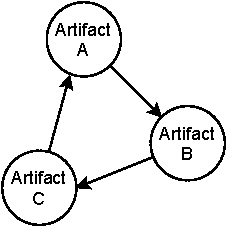
\includegraphics[width=0.5\linewidth]{c4/Fig1a}
        \caption{An example of Cyclic Dependency among artefacts A, B, C.}\label{c2:fig:cd}
    \end{subfigure}
    \hfill
    \begin{subfigure}[t]{0.45\linewidth}
        \centering
        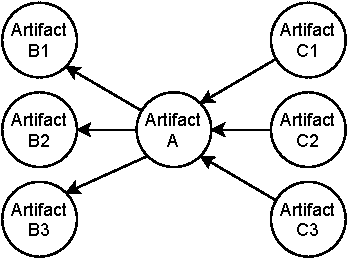
\includegraphics[width=0.7\linewidth]{c4/Fig1b}
        \caption{An example of HL affecting component A, with the afferent (incoming) dependencies on the right and (outgoing) efferent dependencies on the left.}\label{c2:fig:hl}
    \end{subfigure}
    \\
    \begin{subfigure}[t]{0.45\linewidth}
        \centering
        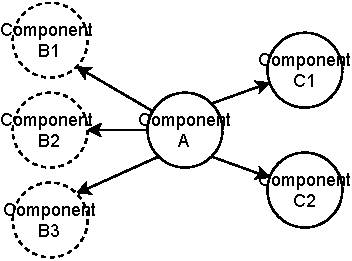
\includegraphics[width=0.7\linewidth]{c4/Fig1c}
        \caption{An example of UD affecting component A. The components that A depends on (Bs and Cs) are shown in the figure too. Components B1 to B3 are less stable than A and represent the majority of A's outgoing dependencies.}\label{c2:fig:ud}
    \end{subfigure}
    \hfill
    \begin{subfigure}[t]{0.45\linewidth}
        \centering
        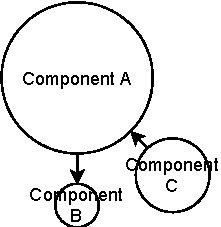
\includegraphics[width=0.5\linewidth]{c4/Fig1d}
        \caption{An example of GC affecting component A. The diameter of A represents its larger size in terms of lines of code w.r.t. other components in the system (B and C).}\label{c2:fig:gc}
    \end{subfigure}
    \caption{Illustration of the four architectural smell types considered in this work.}
    \label{c4:fig:architectural-smells} 
\end{figure}

\subsection{The \textsc{Arcan} tool}\label{c2:sec:arcan}
\textsc{Arcan} parses Java, C, and C++ source code files to create a dependency graph where files, components, classes and packages are all represented using different nodes with different labels. Dependencies, and other relationships between nodes, are represented using edges that connect the dependant to its dependencies with an outgoing, labelled edge (e.g. if artefact \texttt{A} depends on artefact \texttt{B}, then the dependency graph contains a directed edge connecting \texttt{A} to \texttt{B}.). 
The project's structural information contained in the dependency graph is then used to calculate several software metrics (e.g. fan-in, fan-out, instability \cite{Martin2018}, etc.) and then detect architectural smells by recognising their structure in the dependency graph.

Compared to other tools, \textsc{Arcan} uses only software metrics and structural dependencies in order to detect architectural smells. 
This makes \textsc{Arcan} different from tools such as DV8 \cite{Mo2015} (a tool used by related work) which also requires the use of change metrics.
While this type of metrics definitely provide important insights into the maintenance hotspots of the system, they also come with the requirement of needing historical data in order to be used.
This aspect is of particular importance in our case as the version control system adopted by the company we worked with, \emph{did not provide} such information.

Despite the different approaches to detect architectural smells, the two tools,  \textsc{Arcan} and DV8, have some overlap in the detected smells. 
Both tools detect cycles among files and components and both detect hub structures (called \emph{Crossing} by DV8 and Hublike Dependency by \textsc{Arcan}), but DV8 also incorporates historical information for the detection of the latter type of smell.


\subsection{Similarities and differences between code and architectural smells}
Distinguishing between code smells (CS) and AS may not always be easy as different authors have a different understanding of what constitutes one or the other.
In this section, we try to provide a brief explanation about both and clarify the differences between these two concepts.

Code smell is a term first popularised by Kent Beck in the late 1990s \footnote{Read \url{https://wiki.c2.com/?CodeSmell} for more info.} and then further defined by Martin Fowler and Kent Beck himself in the early 2000s \cite{Fowler2002}.
A CS is a sign that the piece of code under inspection requires some changes (i.e. a refactoring) in order to be considered of good quality \cite{Fowler2002}. 
In other words, code smells are symptoms of poor design and implementation choices \cite{Tufano2015}.

The term architectural amell was first adopted by Lippert \cite{Lippert2006} in 2006 to describe a part of the system that required significant refactorings at the architecture level in order to meet the desired quality standards.
To be more specific, Lippert mentions that architectural smells, contrary to code smells, require \emph{large refactorings} in order to be removed from the part of the system they affect and require longer than a day to be applied \cite{Lippert2006}.

Both AS and CS manifest themselves in different forms that are commonly referred to as different \emph{types}.
Some examples of CS types are \emph{Duplicated Code}, \emph{Long Method}, and \emph{Large Class} \cite{Fowler2002}.

Finally, it is important to mention that previous work provides empirical evidence that the AS  considered in this study and the most well-known code smells are \emph{independent} entities and that there is no correlation between the presence of AS and CS \cite{Arcelli2019}.

\subsection{Architectural smell characteristics}\label{c2:sec:smell-characteristics}
An architectural smell characteristic is a property or attribute of an architectural smell instance. 
An architectural smell instance is a concrete occurrence of a type of architectural smell.
For each architectural smell type, one can measure different characteristics. We refer to the characteristics that can be measured for every type of smell as \emph{smell-generic}, whereas we refer to the characteristics that can only be measured for certain types of smells as \emph{smell-specific} characteristics.
The characteristics considered in this work are reported in Table \ref{tab:smell-characteristics}.

\begin{table}[]
    \footnotesize
    \centering
    \caption{The smell characteristics identified by this study. * indicates this study. $^\dagger$ marks characteristics not studied in this study as they are intended as future work.}
    \label{tab:smell-characteristics}
    \begin{tabular}{p{0.035\linewidth}p{0.15\linewidth}p{0.60\linewidth}p{0.025\linewidth}}
    \toprule
    \textbf{Smell} & \textbf{Character.} & \textbf{Description} & \textbf{Ref.} \\ \midrule
    \multicolumn{4}{c}{\itshape smell-generic}\\\midrule
    \multirow{5}{*}{All} & Age & The number of versions affected by the smell. & * \\
     & Overlap Ratio & The ratio of the total number of components of a given smell that also take part in another smell. & * \\
     & Centrality & The importance of the components affected by the smell within the system. Measured using the PageRank of the components in the dependency graph. & (1) \\
     & Size & The number of elements of the system affected by the smell. & * \\
     & Number of edges & The number of dependency edges among the components affected by the smell. & * \\ \midrule
    \multicolumn{4}{c}{\itshape smell-specific}\\\midrule
    \multirow{4}{0.1\linewidth}{CD} & Shape & The cycle shapes as shown in Figure \ref{c2:fig:cycle-shapes}. & (2), (3)\\
    & Average edge weight &  The number of dependencies (weight) between the components affected by the smell. It can be indicative of the difficulty of refactoring the cycle. & (4)\\
     & Number of inheritance edges & The number of edges in the smell that represent an inheritance between components. & (5) \\
     & Affected design level & Whether the cycle is present only at architectural level (among packages) or also at design level (among classes) too. & (3) \\
     & Parent centrality$^\dagger$ & The degree to which a package is at the centre of a cycle with its children sub-packages. & (3)\\ \midrule
     \multirow{2}{0.1\linewidth}{UD} & Instability gap & The difference between the instability of the main component and the average instability of the dependencies less stable than the component itself. & (4) \\
     & Strength (or DoUD (4)) & The ratio between the number of dependencies that point to less stable components and the total number of dependencies of the class. & (4) \\ \midrule
     \multirow{3}{0.1\linewidth}{HL} & Average internal path length$^\dagger$ & Only computed on package HL. The average length of the paths between internal nodes with afferent dependencies and internal nodes with efferent dependencies within the central package. The shorter the length, the more the packages that depend upon the main component and packages that are depended upon by it are connected. & * \\
     & Affected classes ratio$^\dagger$ & Only computed on package HL. The ratio between the number of classes taking part in a dependency relationship with afferent and efferent packages of the main component and the total number of classes in the main component. & *, (6) \\\bottomrule
    \end{tabular}
    (1)\cite{Roveda2018}; (2)\cite{Arcelli2016}; (3)\cite{AlMutawa2014}; (4)\cite{Arcelli2017}; (5)\cite{Laval2012}; (6)\cite{Abdeen2011}
\end{table}

% Why these characteristics?
We decided to focus our analysis on this set of smell characteristics because they are measurable dimensions for the different facets of smells that further quantify the extent to which the smell affects the system; this can  inform developers on how to prioritize refactoring.
Additionally, some of the selected characteristics were developed, studied or discussed by other authors in previous studies, as reported by the Ref. column in Table \ref{tab:smell-characteristics}.

The smell-generic characteristic \emph{Overlap}, \emph{Centrality}, and \emph{Size} are of interest because they are all metrics that are conceptually related to the complexity caused by any instance of a smell in the system. Intuitively, all of them \emph{may} hinder the degree of understandability, extensibility, or generally of maintainability of the components affected by a smell: the more elements a smell has (size), or the more elements of a smell are also involved in other smells (overalp), or the more its elements are interacting with other important components of the system (centrality), the harder it is to fully understand or to refactor the smell. 

\emph{Age}, on the other hand, allows us to track the evolution of the other characteristics over time, identify periods where they are more impactful, or discern eventual correlations between them.

The CD smell-specific characteristics \emph{Shape} and \emph{Average edge weight} are of interest because they are directly related to the complexity of the smell.
The more complex the shape, and the more edges there are between the affected components, the harder the smell is to refactor because more effort is required.
The \emph{Affected design level}, similarly, is important because the cycles present at both package and class level have an impact on two different levels at once.
Finally, the \emph{Number of inheritance edges} characteristic is considered because inheritance edges are considered an indicator of an intentional design choice \cite{Laval2012}, thus intentional cycles that contain a high number of inheritance edges between the components may be more interesting for a developer to inspect.

The UD smell-specific characteristic \emph{Instability gap} and \emph{Strength} are of interest because they are used for the detection of the smell and thus can effectively measure its criticality. The higher the instability gap, the higher the chance the component affected by the smell is changed due to ripple effects \cite{Martin2018}. Likewise, the higher the strength, the higher the chance (because there are more possible components that are prone to a change) a change occurs and propagates to the affected component.

The HL smell-specific characteristics \emph{Affected classes ratio} and \emph{Average internal path length} are of interest because they quantify the involvement of the internal classes in the smell by answering the questions `How many classes belonging to the affected package (out of all package classes) contribute to the smell?' and `How much efferent and afferent packages are actually connected?', respectively.
Intuitively, if the average internal path length is low, it is easier for changes to propagate through the components involved in the smell. And if the efferent and afferent packages are poorly connected (i.e. few paths), the chance a change propagates is small.
In other words, these two characteristics measure the proneness of a HL smell to propagate changes incoming from its dependencies to the components depending upon it.

\section{Case study design}\label{c2:sec:case-study}
The design of the case study follows the guidelines proposed by Runeson et al. \cite{Runeson2012} to conduct and report case studies.
Furthermore, the protocol used to conduct the study and keep track of the changes is based on the template proposed by Brereton et al. \cite{Brereton2008}.

\subsection{Goal and research questions}
The objective of this study is to expand the current knowledge of architectural smells evolution.
Using the Goal-Question-Metric \cite{VanSolingen2002} approach, the objective formulation is:
\begin{quote}\textit{
    \textbf{Analyse} the evolution of individual architectural smells instances throughout the system's history \textbf{for the purpose} of understanding them \textbf{with respect to} their  characteristics and lifespan \textbf{from the point of view of} software architects \textbf{in the context of} open source systems.} 
\end{quote} 
Each one of the research questions that further refine the goal of this study focuses on a different aspect of their evolution: RQ1 studies the evolution trend of each type of smell w.r.t their characteristics, whereas RQ2 studies the survivability (or persistence) of each smell type. 
The two research questions (RQ1 and RQ2) are answered by answering a number of sub-questions (e.g. RQ1a and b for the case of RQ1).

\begin{enumerate}
    \item[\textbf{\textit{RQ1}}] How does each type of architectural smell evolve throughout the system's history?
    \begin{enumerate}
        \item How do the smell characteristics of each smell type (i.e. size, centrality, etc.) evolve over time? 
        \item Is there a correlation between smell characteristics of the same smell type?
    \end{enumerate}
\end{enumerate}
This research question focuses on investigating the evolution of each type of architectural smell through their characteristics and identifying relations among them.
It can provide information for understanding the effects of each type of smell on the system, which can then be used to define refactoring prioritisation rules based on single instances of that type.
Identifying relations is important to avoid using the same information multiple times.
This means that it is necessary to identify eventual correlations among them so that we can determine if we can omit some of the characteristics without losing essential information.

One example of the use of trend as indicator for extra maintenance effort could be the trend of \emph{centrality}, a smell-generic characteristic that measures the degree of connectivity of the elements affected by a smell with the other system's components: the higher the values the more other components are in some way connected to it and thus the more probable for a change to have ripple effects.

\begin{enumerate}
    \item[\textbf{\textit{RQ2}}] How do the different types of smells compare against each other regarding their lifespan?
    \begin{enumerate}
        \item Which types of smells, CD, HL or UD, are more persistent (i.e. are less common to be removed)?
        \item Do the same smell types at package and class level have a different survival probability?
        \item Does the shape of a CD smell affect its lifetime?
        %\item Which types of smells are more likely to generate other smells?
    \end{enumerate}
\end{enumerate}
The aim of this research question is to compare the different types of smells in terms of their survivability. Answering this question could help to define prioritisation rules at the level of smell type.
For example, one could choose to first refactor the types of smells that are more likely to persist longer within the system.

We decided to focus on survivability because it is a time-based measurable dimension of architectural smells, affecting future maintenance: the longer an AS affects a system, the longer the developers and architects will spend extra maintenance effort on the affected components.

\subsection{Case selection}
In this study, we used a set of open source systems known as the Qualitas Corpus (QC) \cite{QualitasCorpus2010}.
We decided to work with open source systems (OSS) for the following reasons: OSS are easy to retrieve and manipulate, the QC has a big variety of different projects ready to be used, and it is easier to develop static analysis tools when there is the possibility to inspect the source code analysed. We consider the extension of our analysis on industrial systems as future work.

The QC has more than 100 projects that can be potentially analysed. We required that projects have more than 15 versions available so to ensure smells have enough time to grow, evolve, and fade, thus limiting  the number of candidate projects to 15.
We also removed EclipseSDK from our selection due to its size causing difficulties during tracking.
The demographics of the selected projects are shown in Table \ref{tab:projects}.

\begin{table}[]
    \centering
    \caption{The projects from the Qualitas Corpus release 20130901e used in this study. A total of 524 versions (both major and minor) were analysed.}
    \label{tab:projects}
    \begin{tabular}{@{}lllll@{}}
    \toprule
    \textbf{Project} & \textbf{\# Versions} & \textbf{First version} & \textbf{Last version} & \textbf{\# Unique AS} \\ \midrule
    Ant & 23 & 1.1 & 1.8.4 & 1211\\
    Antlr & 22 & 2.4.0 & 4 & 1183 \\
    ArgoUML & 16 & 0.16.1 & 0.34 & 3886 \\
    Azureus & 63 & 2.0.8.2 & 4.8.1.2 & 108796 \\
    Freecol & 32 & 0.3.0 & 0.10.3 & 13259 \\
    Freemind & 16 & 0.0.2 & 0.9.0 & 994 \\
    Hibernate & 115 & 0.8.1 & 4.2.2 & 13551\\
    JGraph & 38 & 5.4.4 & 5.11.0.1 & 249\\
    JMeter & 24 & 1.8.1 & 2.9 & 1846\\
    JStock & 30 & 1.0.6 & 1.0.7c & 927 \\
    Jung & 23 & 1.0.0 & 2.0.1 & 238 \\
    JUnit & 24 & 2 & 4.11 & 164 \\
    Lucene & 35 & 1.3.0 & 4.3.0 & 1126 \\
    Weka & 63 & 3.0.1 & 3.7.9 & 2164 \\ \bottomrule
    \end{tabular}
\end{table}

\subsection{Tooling}
To perform the study, we developed a toolchain that allows to mine architectural smells from a series of precompiled Java systems, as illustrated in Figure \ref{c2:fig:data-collection}.
The toolchain is composed of two parts: AS \emph{detection} and AS \emph{tracking}.
\begin{figure}
    \centering
    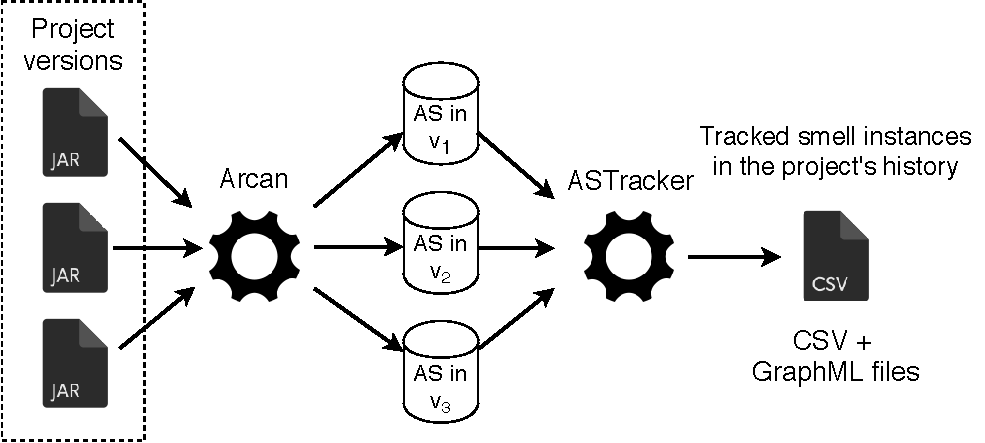
\includegraphics[width=0.8\textwidth]{c2/data-collection-process-pager.pdf}
    \caption{Data collection process and tooling. The data of each individual project was then merged in a single data set.}\label{c2:fig:data-collection}
\end{figure}
\subsubsection{Architectural smell detection}
To identify architectural smells we use \textsc{Arcan}\footnote{\label{fn:Arcan}See \url{https://gitlab.com/essere.lab.public/Arcan}.}, a free Java tool for detecting architectural smells in a system.
\textsc{Arcan} receives as input one, or multiple, JAR files of a single version of a system and outputs a series of CSV files and a GraphML file. The graph file is the dependency graph of the given system extended with nodes denoting architectural smells. The same information as the graph file is contained within multiple CSV files.

\subsubsection{Architectural smell tracking}
In order to perform the study, we needed to track the architectural smells for each pair of consecutive versions of the system, i.e. from $v_1$ to $v_2$, from $v_2$ to $v_3$, and so on.
To this end, we developed a tool, ASTracker\footnote{\label{fn:astracker}See \url{https://github.com/darius-sas/astracker} to access the tool and the data used in this study.}, that performs the following steps: it takes as input multiple versions of a system (the GraphML files produced by \textsc{Arcan}) and maps every smell in each version to its closest successor in the next version, calculates the smell characteristics, and returns the results as CSV and GraphML files.

To perform the mapping of each smell to its successor we use a function $J$ known as \emph{Jaccard similarity index} \cite{Jaccard1912}, defined as
$$J(A, B) = \frac{|A \cap B|}{|A \cup B|}$$
where $A$ and $B$ are the sets of the affected components in two consecutive versions.
The index simply measures the percentage of elements that are shared by the two sets.
The use of this methodology and of the Jaccard index are justified because a smell is defined by the elements it affects: the similarity of the affected sets of elements leads to identifying the successor of a smell.

The comparison among elements in the sets is made using the full name of the classes/packages.
The main advantage of this method is that it avoids name conflicts; however, a renaming in any of the parent packages results in the inability to track the smell in the next version.
Thus, for every smell $k$ in version $v_1$ and for every smell $l$ in version $v_2$, we compute $j_{kl} = J(a(k), a(l))$ which is basically a matrix where the rows are the smells from $v_1$ and the columns are the smells from $v_2$. 
The function $a$ returns the set of elements affected by a smell.
The linking between smells $k$ and $l$ is done using a \textbf{greedy strategy}:
the highest $j_{kl}$ such that $k$ and $l$ have not already been linked with another smell, is the next mapping $k \rightarrow l$ to be created.
The greedy strategy ensures that every smell has been linked with the smell that is most similar to itself, which means formally that only one cell per row and column from the matrix $j$ is selected.
This operation is repeated until there are no more smells left to map or the similarity scores of the remaining ones do not satisfy $j_{kl} \geq \theta$, where $\theta$ is the similarity threshold defined as
\begin{equation*}
\theta = \begin{cases}
     0.67   & \text{ for } |a(k)| > 5 \\ 
     0.60   & \text{ for } |a(k)| \leq 5 \\
    \end{cases}
\end{equation*}

We selected a variable threshold in order to cover the big variance of the function $J$ when $a(k)$ has a relatively small cardinality.
To adjust the thresholds, we consulted all the possible values of $J$ in the case where the two inputs shared all of their elements but only the size changed.
Additionally, we also consulted all the possible values for small input sets sharing a variable number of elements.
The selection of $\theta = 0.60 $ when $|a(k)| \leq 5$ allows for a maximum difference of 3 elements with a smell's successor, allowing the algorithm to be more permissive for smells with fewer elements.
Likewise, a value of $\theta = 0.67$ allows for a reasonable variation when the size of an AS is bigger than 5.

The algorithm only maps smells of the same type, namely CD with CD, UD with UD, and HL with HL.
% \begin{figure}
%     \centering
%     \includegraphics[width=0.45\textwidth, trim = {0.2cm 0.1cm 0.1cm 0.2cm}, clip]{jaccard-scores-bw.png}
%     \caption{Jaccard similarity scores for each pair of smell size (up until 16 and 10). The linking intervals are shown in red squares. In the figure it is assumed that the elements affected are always the same.}\label{c2:fig:jaccard-scores}
% \end{figure}

\section{General results}\label{c2:sec:general-results}
This section introduces some general statistics and insights concerning the data we have collected\footnote{\label{fn:supp-mat}Supplemental material available at \url{http://www.cs.rug.nl/search/uploads/Resources/supp-material-as-evo-icsme19.zip}.}.

\subsection{Smell density}
A good starting point in understanding the evolution of smells is to look at the smell density (\# of smells per component).
As the smell density in a system gets closer to one it means that, on the average,  there is one smell for every component in the system.
Figure \ref{c2:fig:smell-count} shows the density of each smell type across the versions of every system. 

Remarkably, seven projects have a smell density for CD among packages that is either higher or very close to 1 in most of their versions, meaning that it is quite common for developers to create cycles among the packages of the systems, thus increasing the complexity of the system.
It is interesting though to note that the density of CD among classes, in most of the systems, is more or less constant throughout time despite the size of the systems growing (i.e. their ratio remains mostly constant).
In other words, CD smells at class level are constantly introduced by developers as a by-product of the development activities as the system evolves.
This causes also the number of cycles among packages to increase (because some of those cycles will be among classes from different packages), and since the number of classes per package increases over time in most of the systems analysed the smell density on packages is bound to increase as well.
A similar pattern also emerges for UD smells, which are also constantly introduced in the system and have a growing trend.
On the contrary, the number of HL smells stays mostly constant and relatively low (less than 10) over time in all the systems analysed, which is expected as a system has only few components that have a disproportionate number of dependencies.

\vspace{1mm}
\fbox{\begin{minipage}{0.95\linewidth}\small
    \textbf{Takeaway}\\
    Dependencies across packages affected by CD smells become ever tighter as the system ages, making it more difficult over time to reuse them seperately, without importing the whole system.
    This is caused because the cycles among packages grow in number at a higher rate than the number of packages itself.
\end{minipage}}

\begin{figure*}
    \centering
    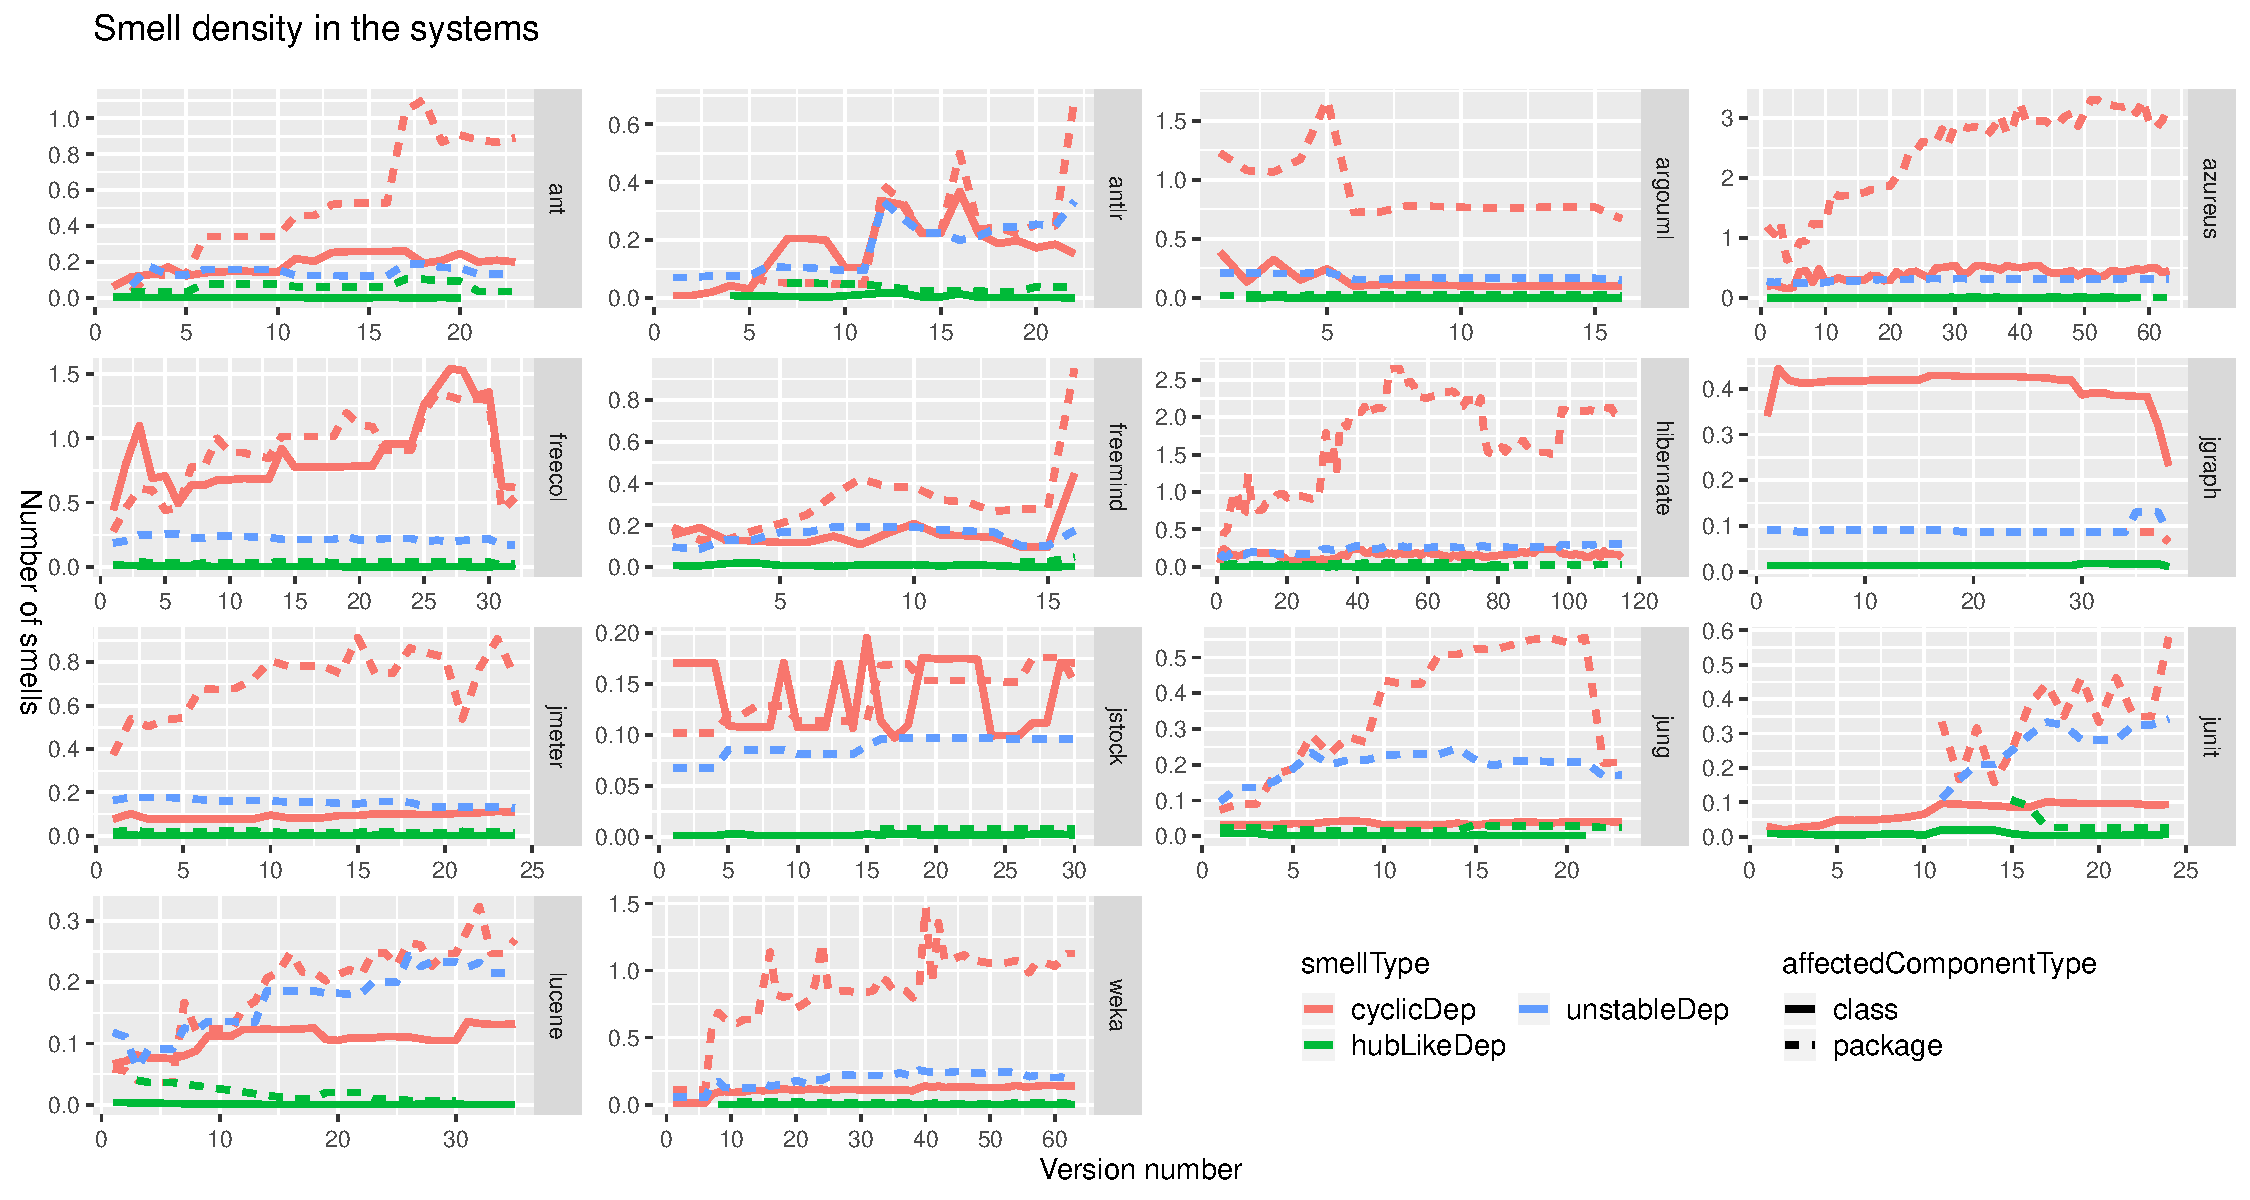
\includegraphics[width=\textwidth]{c2/descriptive-smell-density.pdf}
    \caption{Number of smells in the system divided by total number of classes or packages, depending on the type of the component affected.}\label{c2:fig:smell-count}
\end{figure*}

\subsection{Smell characteristics}\
In this section, we briefly cover some interesting findings on the characteristics mentioned in Table \ref{tab:smell-characteristics}.
One noteworthy finding is the difference in size between smells. HL smells, due to their definition, tend to be usually bigger than the other types of smells, surpassing 100 elements in bigger systems, whereas UD smells are the smallest ones, hardly surpassing 10 elements even in bigger systems.
However, CD and UD smells have higher overlap ratio in general, meaning that trying to refactor a smell with high overlap will entail also dealing with a certain number of other smells.

Concerning UD smells specifically, we note that their instability gap mostly ranges between $-0.1$ and $-0.3$; since these values are relatively close to zero, we argue that they are not very prominent and by slightly improving the instability of few packages, the smell could be removed.
However, the instability gap is also decreasing over time for 50\% of the UD smells detected (more details on this analysis in Section \ref{c2:sec:rq1a-results}), meaning they become more severe over time. 

Finally, we also note that CD smells are mostly at the class level only\footnote{See 'Affected design level' in Table \ref{tab:smell-characteristics} for more details.} (ranging from 60\% to 95\%, depending on the project) or package level only (from 0 \% to 75\%, depending on the project).
A small percentage (less than 3\%) affects class and package level at the same time and an even smaller percentage (1-2\%) switch between levels over time (e.g. they go from class level only to both architectural and class).

\section{Trend analysis (RQ1a)}\label{c2:sec:rq1a-results}
\subsection{Methodology: dynamic time warping}
Analysing the trend of all the characteristics of each smell instance detected in the analysed systems was not a trivial problem to solve, due to its dimensionality (smell instances, time, characteristic).
The approach adopted to solve the aforementioned problem was signal classification: the values assumed by a certain characteristic for a certain smell over time are considered as a signal, then they are compared to a series of predefined signals and a label is assigned to each one of them based on the \emph{distance} from each template.
We used dynamic time warping\footnote{The implementation used for this analysis was provided by the R package \texttt{dtw}.} \cite{Kruskal1983} to warp the signal of each template and stretch it to match the signal one desires to compare it with. 
This technique was previously used by Vaucher et al. to classify the trend of God Classes \cite{Vaucher2009}.

Formally, we can model the problem as follows: for every smell characteristic $C^{k}$ of a certain smell $k$ we consider the different values $C^{k}_i$ as a signal $S$. We then compute the following variables: $h = \max S$; $l = \min S$; and $m = (h+l)/2$.
These three values are then used to build the seven templates, named from $a$ to $g$, as shown in Figure \ref{c2:fig:classification-templates}. For example, temblate (b) is defined as $b = (l, m, h)$.
The templates are re-adjusted for each signal classified.
Finally, the signal is classified by comparing the distance of the signal from each template, and selecting as a label the template name of the closest signal template. 
Specific implementation details can be inspected in the source code.

\begin{figure}[]
    \centering
    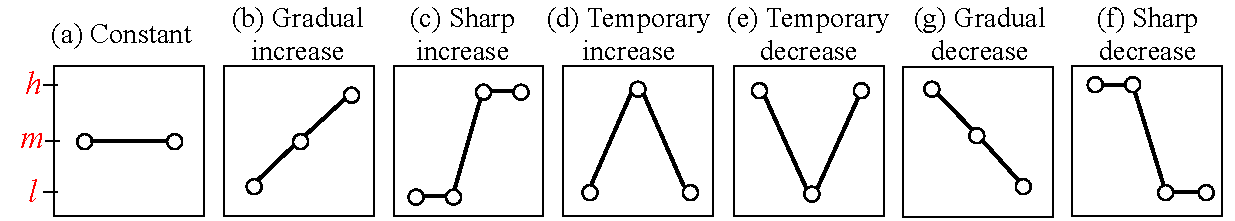
\includegraphics[width=\textwidth,trim={0.2cm 0 0 0},clip]{c2/dynamic-time-warping-min-1line.pdf}
    \caption{Trend evolution classification templates. Figure adapted from the work of Vaucher et al. \cite{Vaucher2009}.}\label{c2:fig:classification-templates}
\end{figure}

Despite the selected templates offering a good variety of possible signal shapes, there may be some cases that are not described well enough by the current selection. For example, signals that vary between two integer values (e.g. 6-7) multiple times, would be classified by the model as a constant signal (i.e. template (a)).
Nonetheless, we deem that the approximation offered by the model when unusual signal curves have to be classified is sufficient for the purpose of this paper for the following reasons:
\begin{itemize}
    \item the templates selected represent simple and general cases, thus they simplify interpretation and analysis;
    \item a signal is classified based on the distance between points from the template and points from the signal itself after being warped, thus the classified signal has at least an internal component that resembles the classification tag (i.e. template) assigned.
\end{itemize}

\subsection{Results}
We performed the aforementioned analysis for all of the numeric characteristics we have recorded.
Hereby we report only the most interesting ones, as there is a large number of data and results that could not realistically fit into this paper.
\paragraph{Size}
Overall, the size of the smells stays constant throughout their evolution, especially in the case of CD and UD. This is shown in Figure \ref{c2:fig:signal-all} where approx. 50\% of the total CD and UD across all systems have a constant trend.
Instead of growing in size, CD smells tend to grow in number, spreading across the system as new elements are added to the system's dependency network (i.e. new classes, packages, etc.).
Nevertheless, there is a fair amount of smells among all the types that exhibit an increasing trend of some kind (types B, C, D).
Specifically, HL smells tend to grow in nearly 65\% (40\% Sharp and 25\% Gradual increase) of the cases. Given its nature, having a hub that keeps getting bigger and bigger through dependencies from more and more classes, or packages, is problematic: that part of the system becomes more complex, it has a lower cohesion and a higher coupling, thus hindering future maintenance activities on it.
It is thus important to \emph{limit the growth} of such smells by redistributing the responsibility of the central component affected by the smell to others.

\paragraph{Number of Edges}
Contrary to size, the number of edges connecting the components affected by a smell have a different trend: they tend to increase.
Specifically, as can be seen in Figure \ref{c2:fig:signal-all}, each smell type exhibits an increasing trend in the number of edges involved in the smell of at least 40\% and up to 80\%.
Additionally, the number of edges between the affected components grows faster than the number of components per se.
Again, this is especially true in the case of HL smells, making them the type of smell that grows faster among the smells studied in this work.
Hublike dependencies are thus an important source of extra maintenance effort, and the number of edges among the affected components of an HL smell can quantify this effort more precisely than the number of affected elements. 
Indeed, this makes sense because an increasing number of edges between components also increases the probability that a change propagates to adjacent components that depend on the component subject to change (as described in Section \ref{c2:sec:arch-smells-hl}).
This fact was also mentioned in a previous work on change proneness metrics of software packages, where the number of method calls (and thus also dependencies) has been used as a change proneness indicator \cite{Arvanitou2015}. Additionally, Martin also links dependencies with change proneness \cite{Martin2018}.

\paragraph{Centrality} 
The centrality metric selected is PageRank \cite{Roveda2018}. We decided to measure the PageRank of a smell as the maximum PageRank value of the affected components and then weight it against the number of elements in each version.
This weighting makes sense because as the system ages, also the number of nodes in the graph used for the calculation of the PageRank increases, scaling down its values, but maintaining the proportions, hence the weighted version allows us to account for this phenomenon.

As one can observe in Figure \ref{c2:fig:signal-all}, as the system and the smells age, the centrality of the smells tends to increase in the vast majority of the cases, especially for CD and HL. On the other hand, UD exhibit more or less the opposite trends.

The results indicate that the component with the highest PageRank (which is very likely to be the central component) in HL smell tends to \emph{``move''} to the centre of the system as the system ages. A similar trend can be observed for CD smells too.
These results confirm a very important assumption for these two types of smells: \emph{AS tend to move to more central parts of the system as they age}. These central parts are also the most important as they have many ingoing dependencies. Consequently, increasingly more maintenance is required for the parts of a system that are affected by CD and HL smells. 

Unexpectedly, for UD one can observe the opposite since most of them exhibit a decreasing trend (types E, F, and G).

\vspace{1mm}
\fbox{\begin{minipage}{0.95\linewidth}\small
    \textbf{Takeaway}\\
    Hublike dependency smells are a better target for refactoring activities in terms of reduction in complexity, future maintenance efforts, and ease of removal for refactoring activities are likely to focus mostly on the central component, by moving functionality elsewhere, rather than on several components as in the case of multiple CD smells.
\end{minipage}}

\begin{figure}[t]
    \centering
    \begin{subfigure}[]{.8\textwidth}
        \centering
        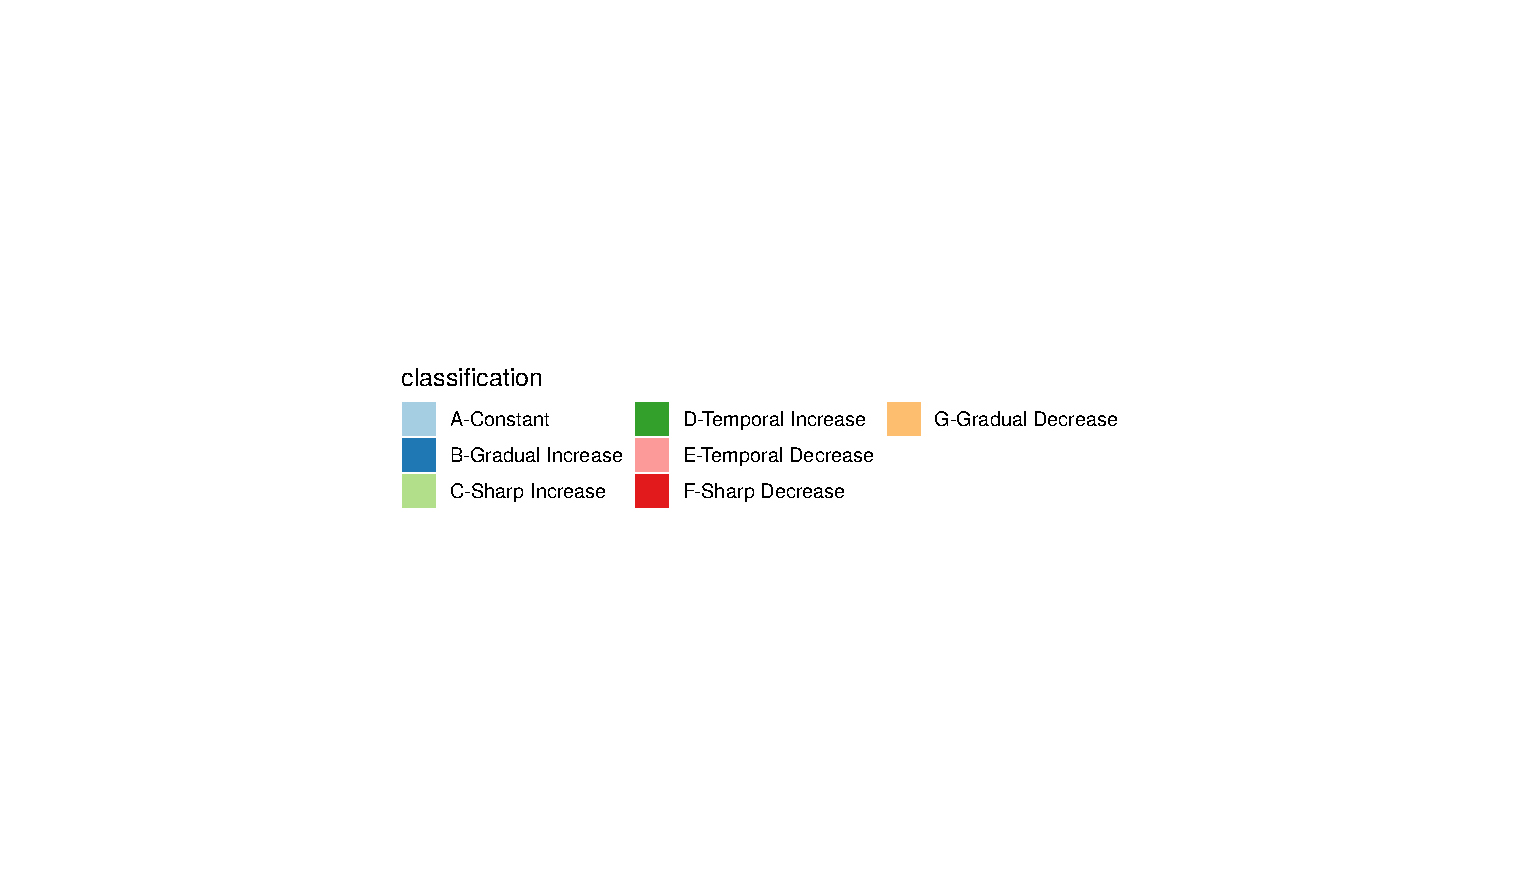
\includegraphics[width=\linewidth,trim={6cm 6cm 6cm 6cm}, clip]{c2/signal-trend-legend.pdf}
    \end{subfigure}
	\hfill \\
    \begin{subfigure}[]{.8\textwidth}
        \centering
        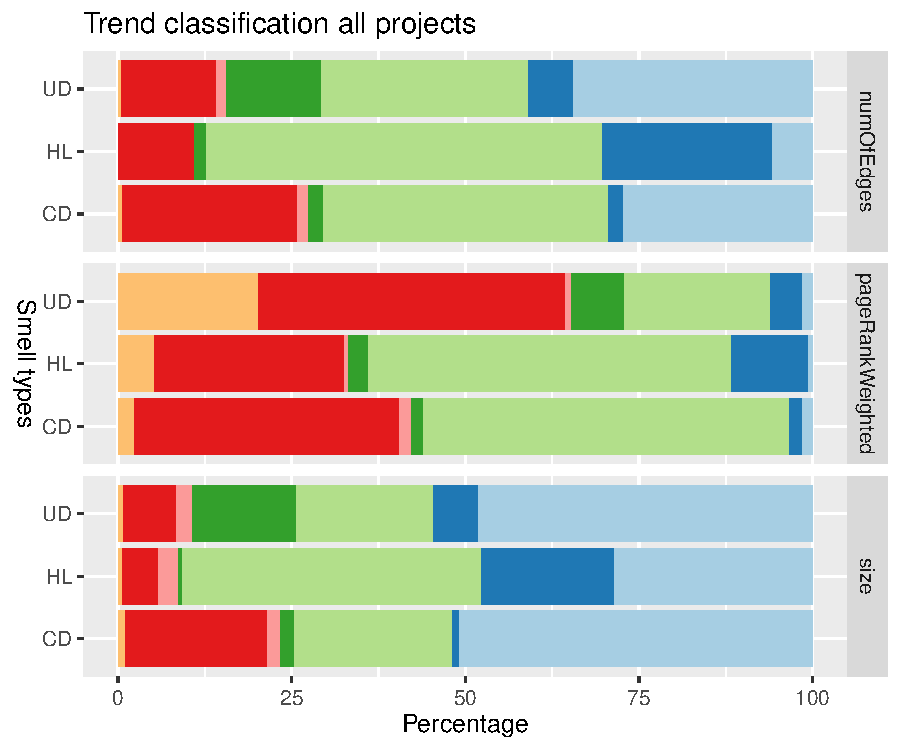
\includegraphics[width=\linewidth]{c2/signal-trend-all-projects-oneplot.pdf}
    \end{subfigure}
    \caption{Signal classification distribution for different characteristics aggregated for all projects as percentages of the total number of smells of that type.} 
    \label{c2:fig:signal-all}
\end{figure}

\section{Correlation analysis (RQ1b)}\label{c2:sec:rq1b-results}
To identify related \textit{pairs of characteristics} for each smell instance of the same type, and for each pair of characteristics, we ran a Spearman correlation test to check for eventual correlations. 
The test was selected because the data is not normally distributed and it is not possible to assume that there is any linear relationship among all the characteristics neither.
The test was performed on each smell instance and only on the pairs of smell characteristics whose both standard deviations were not equal to zero for that instance.
The aggregate test results for all smells were plotted using boxplots (only $p \leq .05$).
The plots are included in the online supplemental material for space reasons.

The characteristics that present a correlation for the majority of the instances detected are the following:
\begin{description}
    \item[Num. of edges $\sim$ Overlap\footnote{The notation $C^1 \sim C^2$ reads `$C^1$ correlates with $C^2$'.}] for smells of type HL and CD at package level. This is expected because of the high smell density at package level (as shown in RQ1a).
    UD, however, do not present such a correlation for these characteristics; this is probably because they usually do not affect central parts of the system, which are more likely to be affected by multiple smells.

    \item[Num. of edges $\sim$ Centrality] for HL smells at class level.
    This was also expected due to the definition of HL (i.e. a component with a lot of incoming and outgoing dependencies, which increases PageRank by definition).
    CD at class level also exhibit a correlation for these two characteristics, but a bit weaker, probably because CD are more frequent among elements near the center.
    %, which is of course expected.

    \item[Num. of Edges $\sim$ Size] strongly for all smells, which is expected.
    
    \item[Overlap $\sim$ Centrality] only weakly. The most prominent correlation is for HL at class level, but is once again expected.
    
    \item[Overlap $\sim$ Size] for CD at class and package level, is also expected, as the bigger the size, the more likely it is that the elements affected are also affected by other smells. The correlations also exist for HL smells, though they are a bit weaker.
          
\end{description}

Number of edges seems to be correlated with a number of characteristics in multiple cases. Despite this result, it is hard to state that, based on this correlation, one should ignore the other characteristics, as these correlations mostly refer to the \textit{majority of the instances} rather than being an absolute gauge of the general case.
In fact, the only pair of characteristics that one can state that are fully correlated for all smell types, independently of the instance, are Size and Number of Edges.
The other correlations are either not valid for all of the smell types, or only a part of the instances analysed show solid evidence of correlation. 

\section{Survival analysis (RQ2a,b,c)}\label{c2:sec:rq2-results}
\subsection{Methodology: the Kaplan-Meier estimator}
The rate of survivability of an architectural smell within a system may drastically vary depending on its type. To establish the rates and compare them among the different projects and smell types, we employed a technique typically used in the biomedical sciences, in product reliability assessment, and also employed to analyse code smell persistence in previous studies \cite{Chatzigeorgiou2014}.
Unlike simple descriptive statistics, such as mean, density functions, and similar, survival analysis also takes into consideration the possibility that a smell continues to affect the system even after the last version included in the analysis.
In the biomedical domain, this event is associated with the patient surviving past the period of the analysis.
%More technically, this type of data is said to be \emph{right-censored}, because the outcome of the treatment could not be measured, generally, due to the conclusion of the study.

The survival analysis is accomplished using the Kaplan-Meier estimator \cite{Kaplan1958}, a non-parametric statistic that estimates the survival probability of a type of smell as the system evolves (new versions are released).
The statistic gives the probability that an individual patient (i.e. smell in our case), will survive past a particular time $t$.
At $t = 0$, the Kaplan-Meier estimator is equal to 1, and as $t$ goes to infinity, the estimator goes to 0. Also, the probability of surviving past a certain point $t$ is equal to the product of the observed survival rates until $t$.

\subsection{Results}
Figure \ref{c2:fig:survival} reports the results of the analysis, i.e. the survival probabilities (a) of different smell types and (b) of different cycle shapes.

\begin{figure}[h]
	\centering
    \begin{subfigure}[]{.7\textwidth}
        \centering
        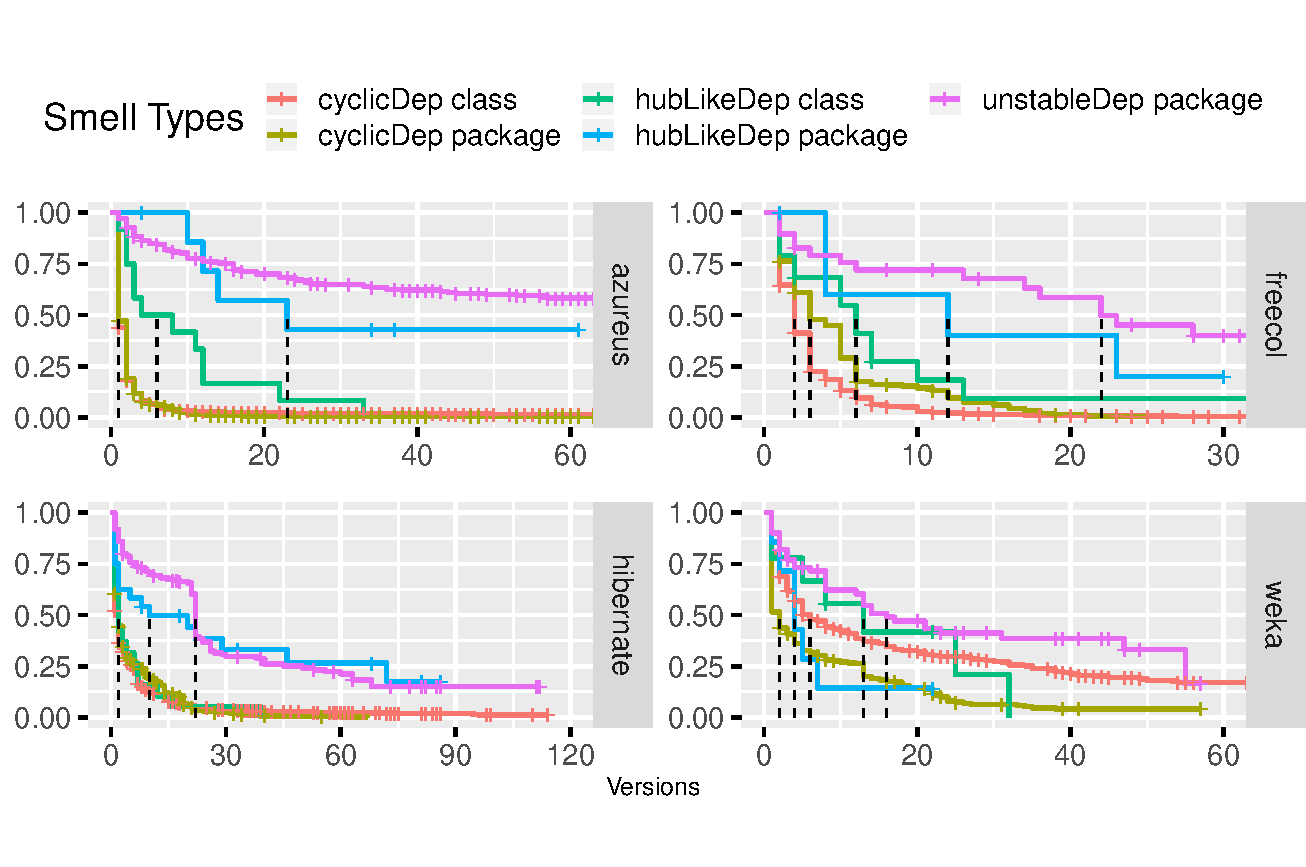
\includegraphics[width=\linewidth, trim={0 0.8cm 0 1cm}, clip]{c2/survival-probabilities-selection.pdf}
        \caption{Smells of different types affecting classes or packages.}
        \label{c2:fig:surival-smells} 
    \end{subfigure} \hfill \\
    \begin{subfigure}[]{.7\textwidth}
        \centering
        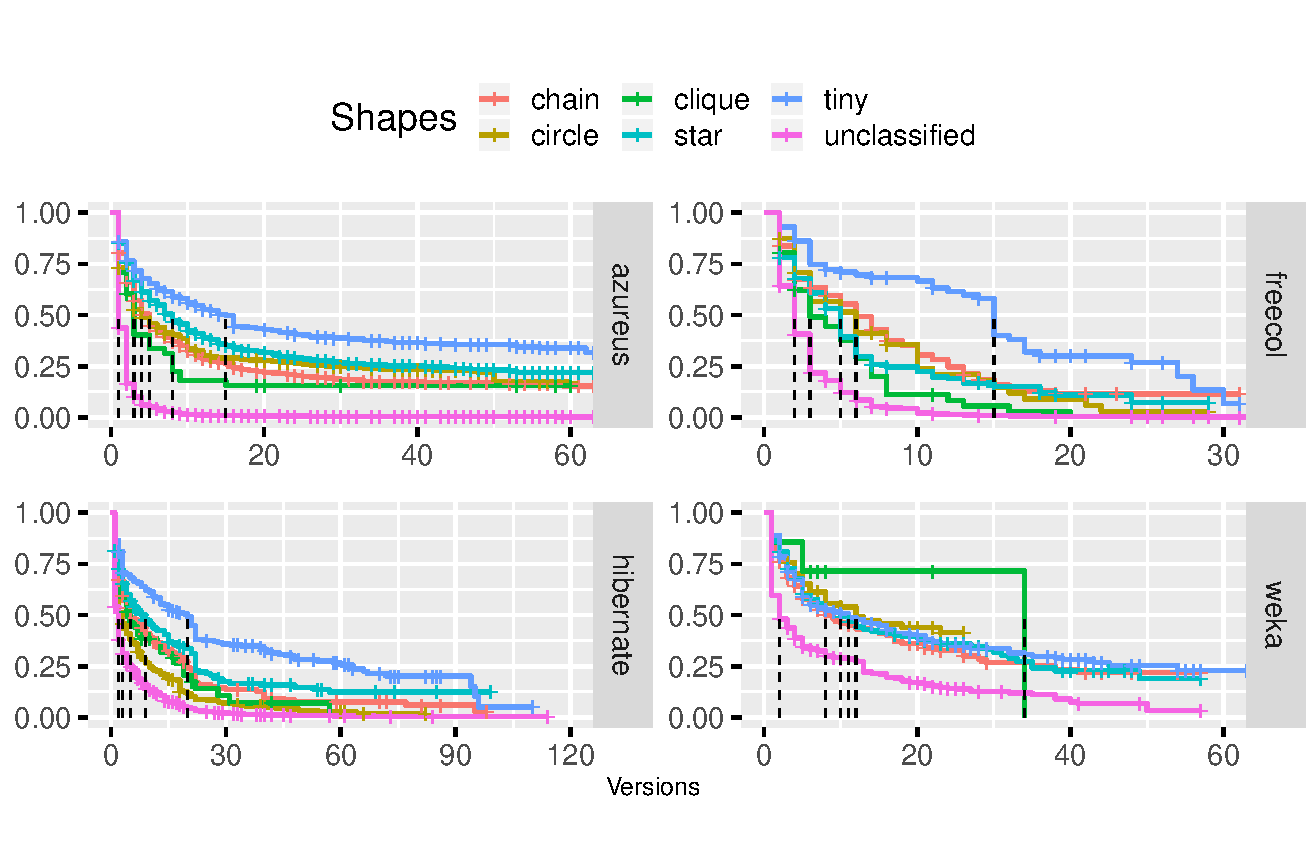
\includegraphics[width=\linewidth, trim={0 0.8cm 0 1cm}, clip]{c2/survival-probabilities-shapes-selection.pdf}
        \caption{Cyclic dependencies of different shapes.}
        \label{c2:fig:survival-shapes} 
    \end{subfigure}
    \caption{Survival probability $p$ up until any time $t$. $p = 0.50$ is represented by a vertical dashed line. Only a selection of systems is shown here for the sake of readability. The full plot is available in the online supplemental material.}
    \label{c2:fig:survival}
\end{figure}

\subsubsection{Survival probabilities of different smell types (RQ2a,b)}
One pattern that emerges from Figure \ref{c2:fig:survival}a is that CD smells fade much quicker than the other types of smells in almost all of the systems and have a very small probability to persist within the system for a long time.
We conjecture that the cycles that persist the most are the cycles among the fundamental components of the system; these are very unlikely to change after the core development activities for that part settle down and new functionalities attract the effort of developers.
Moreover, we also note that cycles only have a \emph{50\% chance} to stay within the system for more than 4-5 releases. Furthermore, cycles among classes persist a little longer within the system than cycles among packages, probably because classes taking part in cycles at design level only might have a stronger coupling with each other than packages.

Another pattern that emerges is that UD is the most persistent type of smell, being the one with the highest survival probability in the long run.
Its survival probability is so high that in some systems it never falls below 50\%, even when there are a lot of versions such as in the case of Azureus.
Moreover, it also decreases at a much slower rate than the other types of smells, making it an ideal target for refactoring to avoid extra maintenance effort in the long run.

HL smells, are more or less in between the other two smell types. They exhibit a similar decrease rate in survival probability as CD smells but eventually end up surviving for more releases. However, this pattern does not hold for all the projects, and in some cases, HL smells end up being removed within fewer versions than CD.
This trend holds true especially for HL at the class level, which tend to decay much faster than HL at the package level.
Thus, it is reasonable to state that HL at package level can be prioritised over HL at class level as they have a higher chance of requiring extra maintenance over time.
In general, from this analysis one can conclude that package level smells, such as UD and HL on packages, tend to last a little bit longer than class level smells, implying that smells at the package level are potentially more impactful on maintenance efforts than smells affecting classes only.

\fbox{\begin{minipage}{0.95\linewidth}\small
    \textbf{Takeaway}\\
    The refactoring prioritisation should \textbf{not focus on cyclic dependencies} that were recently introduced, as it is very likely that they will disappear within the next few releases because they are less likely to influence the maintenance effort on the long term.
    Instead, refactoring should first focus on either UD smells or HL smells among packages as they exhibit higher persistence rates.
    This also confirms that most circular dependencies are not critical \cite{AlMutawa2014}.
\end{minipage}}\\
\subsubsection{Survival probability of different CD shapes (RQ2c)}
Concerning the different shapes of CD smells, Figure \ref{c2:fig:survival-shapes} shows how different shapes persist within the system.
The results show that the most pervasive shape in most systems are tiny shapes. This makes sense as tiny shapes are composed by only two elements and there might be multiple dependency edges between the two elements; thus the probability of a tiny cycle to break is smaller than shapes with multiple elements.
Additionally, tiny cycles are easier to understand and may also be intentionally designed as such.

On the other hand, the other, more complex, shapes are less \emph{resilient} (i.e. they disappear faster than tincy cycles) and there is very little difference between different shape types, making it hard to formulate any solid proposition on their survivability. In order for these complex shapes to persist, they must affect parts of the system that have a solid conceptual connection; otherwise they do not persist long within the system.

Regarding instead the cycles \textsc{Arcan} could not classify into definite shapes, they have a more consistent trend and disappear quicker than all other shapes.
A possible explanation could be related to their nature: we conjecture that this type of cycle is mostly random and caused by casual relationships among components that tend to connect multiple uncomplete cycles into a single one, possibly overlapping with other cycles as well.
Thus these very volatile edges that interconnect multiple parts of a system have a high chance of getting changed because they are individual edges, and if one of these edges is removed, the whole cycle breaks.
This is also evident from the clear difference in survival probability between the unclassified shapes and the complex shapes (circle, chain, clique, star).

\fbox{\begin{minipage}{0.95\linewidth}\small
    \textbf{Takeaway}\\
    We suggest that tiny shapes should not to be prioritised during refactoring even though it is the most persistent one, as it may be the \textbf{result of intentional design} (false positives).
    Refactoring activities, instead, should prioritise old cycles with complex shapes that  are more likely to affect important parts of the system, and thus that are more likely to incur extra maintenance effort.
\end{minipage}}
%IMPORTANT ADDITION FOR CAMERA READY
%We hypothesise that this is imputable to the highly connected network that a system grows into as more and more components (due to new functionality, probably) are added. Hence, as soon as a single edge, or node, changes within this intricate network, one or multiple cy-cles are broken or created, which is also confirmed by the high overlapping between smells and the ‘less-constant’ trend of the characteristic number of edges. This has an important consequence on the smells that one should consider refactoring, both type-wise and in-stance-wise.

%\section{Discussion}\label{c2:sec:discussion}

% Smell density constant to project size
% Smells tend to move to more central parts of the system
% CD stable in size, but grow rapidly in number
% CD smells decay much quicker than other smell types
% Tiny shapes are most persistent probably due to the ease of creating them as intentional design
% Unclassified shapes, and CD in general, may be the result of casual relations among components that complete/finish bigger cycles, thus explaining their volatility.
% UD smells are the most persistent ones
% HL smells are in the middle: class-level ones tend to survive more like CD, whereas package level ones tend to survive more like UD.
% HL stable in number, grow rapidly in size

% Give general interpretation of results
% Implication for practitioners and researchers
% Pillar components
% Architectural index should weight the age based on survivability rates (i.e. CDs younger than 5 versions are only weighted 0.5, like their survival probability)

\section{Threats to validity}\label{c2:sec:threats}
We identified the possible threats to validity for this study and categorised them using the classification proposed by Runseson et al. \cite{Runeson2012}: \emph{construct validity}, \emph{external validity}, and \emph{reliability}.
Internal validity was not considered as we did not examine causal relations \cite{Runeson2012}.

\paragraph{Construct validity}
This aspect of validity reflects to what extent this study measures what it is claiming to be measuring \cite{Runeson2012}.
In this study, we aim at measuring the evolution of architectural smells instances and understand them depending on their type and different characteristics.
We developed a case study using a well-known protocol template \cite{Brereton2008} that was reviewed by the three authors and an external researcher in several iterations to ensure that the data to be collected would indeed be relevant to the research questions.

A possible threat to construct validity  is the correctness of the tracking algorithm that might be incorrect or not cover some special cases, such as the renaming of the affected components.
To mitigate this threat, we manually validated the tracking results for one of the projects considered in this study (Antlr) and fixed any issues we found during our inspections.

Another threat concerns the detection of the smells considered in this project which depends on the implementation offered by \textsc{Arcan}. This is partially mitigated, as the \textsc{Arcan} tool has already been used and evaluated in a number of studies \cite{Arcelli2016, Biaggi2018}.

Finally, the last threat we identified is the relatively \emph{long}, and \emph{variable} periods of time in between the versions analysed for each project. This problem may have caused the prevalence of `sharp' classification in the trend analysis over the `gradual' ones.
We mitigated this threat by limiting the importance we attribute to the specific type of the trend and focusing mostly on its nature (i.e. increase/decrease) and by also including projects with a strict release schedule (e.g. Hibernate).

\paragraph{External validity}
This aspect of validity reflects to what extent the results obtained by this study are generalisable to similar contexts.
The second one regards the projects we used to collect the necessary data. These projects were all open-source Java systems, Hence, it is not possible to generalise these results to industrial projects or projects written in a different programming language.
However, we addressed this threat by adopting a collection of systems (the Qualitas Corpus) specifically intended for scientific analyses and tried to include as many \emph{projects} and \emph{versions} as possible in order to increase the sampling size of the population analysed.
Our findings can thus be generalised to other Java projects of similar size and history that have an active open source community backing the development efforts.

\paragraph{Reliability}
Reliability is the aspect of validity focusing on the degree to which the data and the analysis are dependent on the researcher performing them.

The data and the tools used in this study are freely available online to allow other researchers to assess the rigour of the study or replicate the results using the same data set or even on a different set of projects.

The reliability of the findings is guaranteed by the fact that all the intermediary results were inspected by a second researcher during all the data analysis process.
The analysis was also performed using well-established techniques already used in previous work for analysing similar artefacts (code smells) as well as also in different fields (e.g. survival analysis, in the biomedical sciences field).


% TODO
\section{Conclusions and future work}\label{c2:sec:conclusions}
This study has investigated the evolution of instability architectural smells in the context of open source systems with respect to their characteristics and persistence.
We presented multiple findings and practical implications useful both for practitioners and researchers that can help them improving the strategies for reducing long term maintenance efforts by managing architectural smells.
% In particular, we found that cyclic dependencies tend to persist within the system for quite a short number of releases mostly due to the vast amount of links among nodes that may randomly appear or disappear, creating or destroying cycles. Nonetheless, cycles with more structured shapes seem to persist longer.

% We also provided evidence on how smells `move' to the centre of the system as they age and how their complexity increases mostly on the number of edges rather than on the number of elements affected, despite these two characteristics being correlated.

As future work, we plan to extend our tooling to mine architectural smells directly from Git repositories, thus allowing us to link the current information to code churn and investigate the effects of smells on change rates.

\section*{Acknowledgements}
This work was supported by the European Union's Horizon 2020 research and innovation programme under grant agreement No. 780572 SDK4ED (\url{https://sdk4ed.eu/}).
